A necessidade da busca de métodos que poderiam vir a ajudar na evolução do processo de construção de software, culminaram com o desenvolvimento da Engenharia de Software, disciplina que traz consigo métodos e técnicas que ajudam na administração da complexidade inerente do software. Contudo, apesar de inegáveis avanços, ainda existem pontos obscuros, sendo certamente requisitos de software um destes pontos.
No ano de 1979, o Gouvernment Accouting Office (GAO) nos USA publicou um relatório no qual afirmava que menos de 2% (dois por cento) dos investimentos feitos no desenvolvimento de software resultaram em um software que atendia seus requisitos (2).
Tal ineficiência no alcance da satisfação dos clientes referentes ao produto final de software, resultaram no surgimento, desenvolvimento e definição de processos de desenvolvimento de software, com o objetivo de aumentar a produtividade e diminuir os riscos de um projeto(3).
Dentre estes processos, encontram-se o processo cascata, o interativo, o espiral, o incremental, entre outros, que podem ser aplicados à soluções que melhor se encaixam em seus princípios e contextos. Para o presente projeto, foi proposta uma solução baseada nas Metodologias Ágeis (MAs): Abordagem que tem como objetivo principal garantir a entrega de produtos em um menor prazo, com maior qualidade e satisfazendo às necessidades dos clientes através da aplicação da produção enxuta para desenvolvimento de software, atacando os desafios emergentes de contextos dinâmicos (4). Baseado na análise do processo, foi determinada a utilização do processo SAF para o presente projeto, que será sucintamente descrito subsequentemente.

\section {Scaled Agile Framework (SAF)}

Tendo sua origem nas metodologias e filosofias ágeis, o SAF é um processo criado inicialmente para se adaptar ao contexto empresarial, trazendo a possibilidade de realizar entregas rápidas e com proximidade do cliente, alinhando constantemente com a expectativa do mesmo e adaptando constantemente o projeto às mudanças de requisitos do cliente.
O SAF tem foco  no produto em detrimento da documentação e nas pessoas envolvidas no processo, aproximando estas e trazendo o cliente como membro efetivo da equipe. Este tem papel fundamental na tomada de decisões no processo do desenvolvimento do projeto.
Tais práticas corroboram uma maior adaptatividade à mudanças, tendendo a amenizar riscos no processo de execução do projeto, principalmente pela proximidade entre equipe e cliente (BOEHM, 2002) (1)
O SAF é baseado nos princípios Ágeis, que se baseiam nos nove princípios seguintes:


\begin{itemize}
\item Adotar uma visão sistêmica
\item Entendemos a economia da cadeia de valor
\item Desenvolvemos sistemas iterativamente e incrementalmente
\item Integramos e testamos frequentemente; adaptamos imediatamente
\item Gerenciamos riscos e a eficácia através de ciclos de aprendizado rápido e síncrono
\item Facilitamos o fluxo: limitamos o trabalho em execução, reduzimos o tamanho do lote e gerenciamos a duração da fila
\item Sincronizamos entre os domínios o planejamento e a colaboração
\item Baseamos marcos na avaliação objetiva dos sistemas de trabalho
\item Desbloqueamos a motivação intrínseca dos trabalhadores do conhecimento
\item Descentralizamos a tomada de decisão
\end{itemize}

A natureza particular dessa proposta é a ênfase que o framework dá ao gerenciamento de requisitos, trazendo novos conceitos nesta área, como histórias (user stories), temas (themes) e épicos (epics). Conceitos que ampliaram a forma de capturar requisitos, melhor adequados à ênfase em colaboração, flexibilidade e iterações mais curtas no projeto. (5)

\begin{figure}[H]
		\centering
		\caption{SAF}
		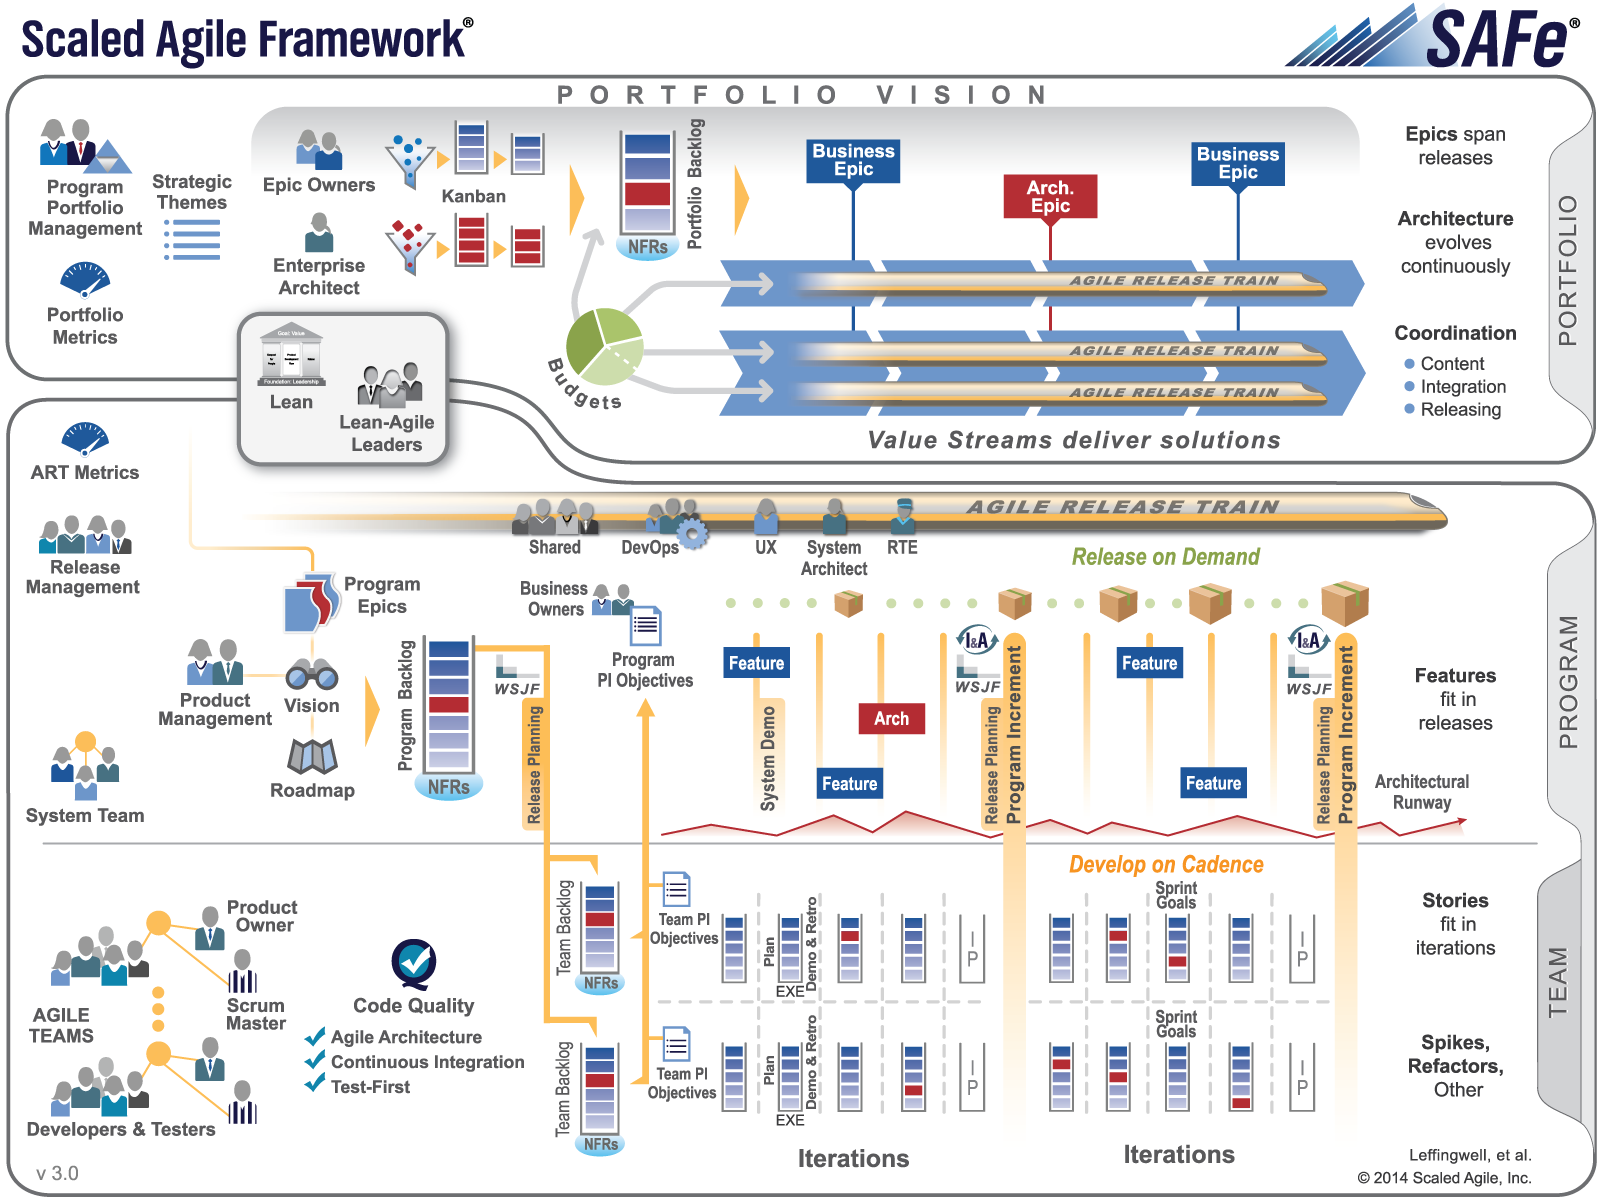
\includegraphics[width=\textwidth]{figuras/SAF}
		\label{img:SAF}
\end{figure}



\section {Modelo de Maturidade}

O modelo de maturidade foi desenvolvido para auxiliar a execução de atividades que envolvam processos. Ele funciona como um guia em que a organização deve-se  espelhar, realizar um plano , a fim de chegar em um nível de excelência. A exigência da contínua melhora dos projetos é o que torna como necessidade este gerenciamento de maturidade.(6)
Pode-se entender que ao utilizar o modelo de maturidade, a organização envolvida terá vários benefícios como: mais produtividade das equipes, redução de custos, riscos do projeto minimizados, aumento do retorno de investimento e qualidade no produto entregue. (7)

\subsection {MPS.BR}

O MPS.BR (Melhoria do Processo de Software Brasileiro) tem o objetivo de melhorar a qualidade dos processos de software, principalmente das micro, pequenas e médias empresas. Ele baseia-se no CMMI (Capability Maturity Model - Integration) e é constituído pelas normas: NBR ISO/IEC 12207 – Processo de Ciclo de Vida de Software, pelas emendas 1 e 2 da norma internacional ISO/IEC 12207 e pela ISO/IEC 15504 – Avaliação de Processo. (10)
Ele está dividido em três modelos: Modelo de Referência (MR-MPS), Método de Avaliação (MA-MPS), Modelo de Negócio (MN-MPS) como pode ser visto na (Figura \ref{img:mps2}).

\begin{figure}[H]
		\centering
		\caption{Programa MPS.BR}
		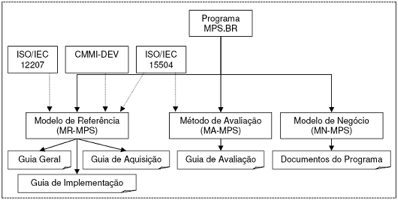
\includegraphics{figuras/mps2}
		\label{img:mps2}
\end{figure}

\begin{itemize}

\item MR-MPS[H]

O modelo de referência para melhoria do processo de software é dividido em vários níveis de maturidade como pode ser visto na (Figura \ref{img:MR-MPS2}).

\begin{figure}
		\centering
		\caption{Níveis de maturidade MR-MPS}
		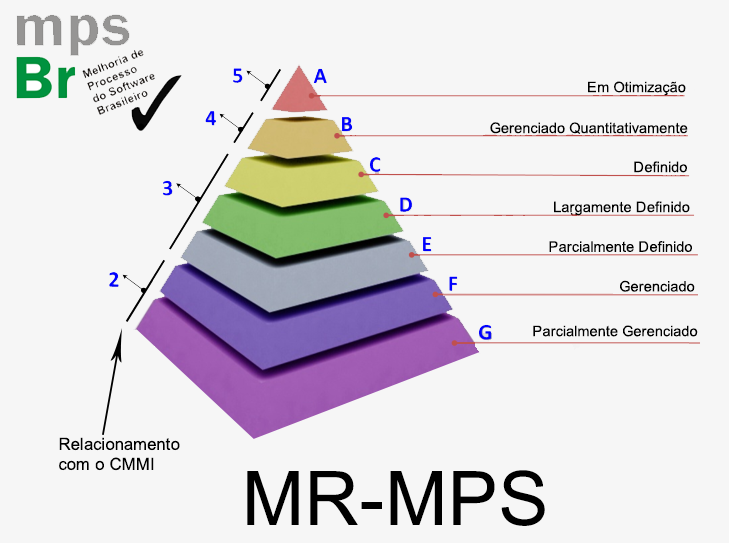
\includegraphics[width=\textwidth]{figuras/MR-MPS2}
		\label{img:MR-MPS2}
\end{figure}

“Os níveis de maturidade estabelecem patamares de evolução de processos, caracterizando estágios de melhoria da implementação de processos na organização. O nível de maturidade em que se encontra uma organização permite prever o seu desempenho futuro ao executar um ou mais processos.” (10)

Em cada nível de maturidade da figura \ref{img:MR-MPS2}  são analisados os processos fundamentais, processos organizacionais e processos de apoio.

Processos Fundamentais:

\begin{itemize}
\item Aquisição
\item Gerência de requisitos
\item Desenvolvimento de requisitos
\item Solução técnica
\item Integração do produto
\item Instalação do produto
\item Liberação do produto
\end{itemize}

Processos Organizacionais:

\begin{itemize}
\item Gerência de projeto
\item Adaptação do processo para gerência de projeto
\item Análise de decisão e resolução
\item Gerência de riscos
\item Avaliação e melhoria do processo organizacional
\item Definição do processo organizacional
\item Desempenho do processo organizacional
\item Gerência quantitativa do projeto
\item Análise e resolução de causas
\item Inovação e implantação na organização
\end{itemize}

Processos de apoio:

\begin{itemize}
\item Garantia de qualidade
\item Gerência de configuração
\item Validação
\item Medição
\item Verificação
\item Treinamento
\end{itemize}

A engenharia de requisitos se encontra nos níveis D e G, Largamente Definido e Parcialmente Gerenciado, respectivamente.


\textbf{Nível G}

Gerência do Projeto e Gerência de Requisitos compõem o nível G de maturidade.
A finalidade do processo de Gerência de Requisitos é gerenciar os requisitos e componentes do produto do projeto. Além de identificar as inconsistências entre os requisitos, planos e produtos do projeto.(12)

Resultados esperados:

\textbf{GRE 1} - Comunicação constante com os fornecedores de requisitos;

\textbf{GRE 2} - Os requisitos são compreendidos;

\textbf{GRE 3} - Requisitos são aceitos;

\textbf{GRE 4} - Comprometimento com os requisitos;
\textbf{GRE 5} -Rastreabilidade entre os requisitos, planos do projeto e produtos do trabalho;
\textbf{GRE 6} - São corrigidas as inconsistências entre os requisitos, planos e produtos do projeto;
\textbf{GRE 7} - Ao longo do projeto as mudanças nos requisitos são gerenciadas.

\textbf{Nível D}

Neste nível acontece o Desenvolvimento de Requisitos, Integração do Produto, Solução Técnica, Validação, e Verificação. (12)

Os requisitos são estabelecidos em conformidade com o cliente.

Resultados esperados:

\textbf{DRE 1} - São identificadas as necessidades, expectativas, restrições e requisitos de interface do cliente;
\textbf{DRE 2} - Requisitos funcionais e não-funcionais são estabelecidos;
\textbf{DRE 3} - Requisitos são refinados;
\textbf{DRE 4} - Conceitos operacionais e cenários são desenvolvidos;
\textbf{DRE 5} - As funcionalidades são desenvolvidas;
\textbf{DRE 6} -Requisitos são avaliados para assegurar as necessidades dos interessados;
\textbf{DRE 7} - Requisitos são validados.

\item {MA-MPS}

É o método que permite a avaliação segundo o modelo MPS, seguindo o processo de avaliação e método de avaliação MPS, e características de qualificação dos avaliadores. (10)

O processo de avaliação é constituído por 4 etapas :

\begin{itemize}
\item Contratar a avaliação;
\item Preparar a realização da avaliação;
\item Realizar a avaliação;
\item Documentar os resultados da avaliação.
\end{itemize}

\item {MN-MPS}

O Modelo de Negócio tem o objetivo de credenciar as instituições que seguirem o Modelo de Referência (MR-MPS), Método de Avaliação (MA-MPS), tiverem experiência em processos de software e possuírem estratégias de implementação do modelo e treinamento dos consultores. (10)


\end{itemize}



\section {Mapeamento do Contexto vs Abordagens}
